\documentclass[11pt,a4paper]{article}
% Configuración común del informe.
\usepackage[T1]{fontenc}
\usepackage[utf8]{inputenc}
\usepackage[spanish,es-noquoting]{babel}
\usepackage{newtxtext,newtxmath}   % Times New Roman (texto y ecuaciones)
\usepackage{graphicx}
\usepackage{amsmath}
\usepackage{booktabs}
\usepackage{caption}
\usepackage{subcaption}
\usepackage[margin=2.5cm]{geometry}
\usepackage{siunitx}
\usepackage{hyperref}

\hypersetup{hidelinks}
\sisetup{output-decimal-marker={,}, separate-uncertainty=true}

% "Figura 1: ..." y "Tabla 1: ..." con la etiqueta en negrita.
\captionsetup{labelfont=bf, font=small, width=0.9\textwidth}

% Abreviaturas de referencia cruzada usadas en el texto.
\newcommand{\figref}[1]{Fig.~\ref{#1}}
\newcommand{\ecref}[1]{Ec.~(\ref{#1})}
\newcommand{\tabref}[1]{Tabla~\ref{#1}}

% Vectores: negrita sin itálica. Escalares: itálica sin negrita.
\renewcommand{\vec}[1]{\mathbf{#1}}

% Babel en español rotula las tablas como "Cuadro"; el informe usa "Tabla".
\addto\captionsspanish{\renewcommand{\tablename}{Tabla}}


% ---------------------------------------------------------------
% Datos de la portada. Completar con los del grupo antes de entregar.
% ---------------------------------------------------------------
\newcommand{\numerogrupo}{XX}
\newcommand{\comision}{S}
\newcommand{\integrantes}{%
  Apellido, Nombre \\ Apellido, Nombre \\ Apellido, Nombre%
}

\begin{document}

% =========================== PORTADA ===========================
\begin{titlepage}
\centering

\includegraphics[width=0.42\textwidth]{figuras/logo-itba.png}\\[1.4cm]
{\large 72.25 Simulación de Sistemas}\\[0.5cm]
{\large Trabajo Práctico N.º 2}\\[1.8cm]
\rule{\textwidth}{0.6pt}\\[0.5cm]
{\LARGE\bfseries Autómatas celulares fuera de red:\\[0.25cm]
transición al orden colectivo en bandadas\\[0.25cm]
de agentes autopropulsados\\[0.4cm]}
\rule{\textwidth}{0.6pt}\\[1.6cm]
{\large Grupo \numerogrupo{} --- Comisión \comision}\\[1.0cm]
{\large \integrantes}\\[\fill]
{\large 4 de septiembre de 2026}
\end{titlepage}

\tableofcontents
\newpage

% ========================= INTRODUCCIÓN =========================
\section{Introducción}

Un conjunto de individuos que se desplazan de forma autónoma puede desarrollar
movimiento colectivo sin que exista un líder ni una señal global que coordine al
grupo. Bandadas de aves, cardúmenes y colonias bacterianas exhiben este
comportamiento, y una parte considerable del interés que despierta reside en que
el orden global emerge de reglas de interacción estrictamente locales.

El modelo introducido por Vicsek et~al.~\cite{vicsek1995} captura ese fenómeno
con una formulación mínima: partículas puntuales que se mueven con rapidez
constante y que, en cada paso de tiempo, adoptan la dirección promedio de sus
vecinas dentro de un radio de interacción, perturbada por un ruido de amplitud
controlada. Pese a su sencillez, el sistema presenta una transición entre un
régimen desordenado, donde las direcciones individuales se cancelan, y un
régimen ordenado, donde las partículas se desplazan de forma coherente. El
parámetro de ruido $\eta$ actúa como variable de control de esa transición.

La regla de alineamiento no es, sin embargo, la única posible. El modelo del
votante~\cite{loscar2021} reemplaza el promedio sobre todo el vecindario por la
copia de la dirección de un único vecino elegido al azar. Ambas reglas comparten
la información disponible —las direcciones de las partículas cercanas— pero la
procesan de manera distinta: una promedia y la otra imita. Esa diferencia, que
parece menor, altera de forma sustancial cómo el ruido destruye el orden y a
partir de qué valor de $\eta$ el sistema deja de estar polarizado.

Este trabajo implementa ambas reglas sobre la misma dinámica y las compara
cuantitativamente. El estudio se organiza en torno a dos observables: la
polarización $v_a$, que mide el grado de alineamiento global, y la fracción de
partículas contenidas en la componente conexa más grande de la red de
interacción, $S$, que mide cuán agrupado está el sistema en el espacio. El
análisis conjunto de ambos permite distinguir el orden en las direcciones del
orden en las posiciones, y establecer en qué medida uno condiciona al otro.

% ============================ MODELO ============================
\section{Modelo}
\label{sec:modelo}

\subsection{Dinámica común}

El sistema consta de $N$ partículas puntuales confinadas en una caja cuadrada de
lado $L$ con condiciones periódicas de contorno. La partícula $i$ queda descrita
por su posición $\vec{r}_i(t)$ y por el ángulo $\theta_i(t)$ que fija la
dirección de su velocidad. La rapidez $v$ es idéntica para todas las partículas
y constante en el tiempo, de modo que la velocidad es
%
\begin{equation}
\label{eq:velocidad}
\vec{v}_i(t) = v\left(\cos\theta_i(t),\; \sin\theta_i(t)\right).
\end{equation}
%
La posición evoluciona por integración explícita de la \ecref{eq:velocidad}
usando la velocidad del paso corriente,
%
\begin{equation}
\label{eq:posicion}
\vec{r}_i(t+\Delta t) = \vec{r}_i(t) + \vec{v}_i(t)\,\Delta t,
\end{equation}
%
y el resultado se reduce al intervalo $[0,L)$ en cada coordenada para imponer la
periodicidad. Como todas las partículas tienen el mismo módulo de velocidad, la
única variable dinámica no trivial es el ángulo.

El vecindario de interacción de la partícula $i$ es el conjunto
%
\begin{equation}
\label{eq:vecindario}
\mathcal{N}_i(t) = \left\{\, j \;:\; d\!\left(\vec{r}_i(t), \vec{r}_j(t)\right) \le r_c \,\right\} \cup \{i\},
\end{equation}
%
donde $d(\cdot,\cdot)$ es la distancia mínima bajo condiciones periódicas y
$r_c$ el radio de interacción. La partícula se incluye a sí misma en su
vecindario, tal como en la formulación original~\cite{vicsek1995}; esto garantiza
que $\mathcal{N}_i$ nunca sea vacío y que una partícula aislada conserve su
dirección salvo por el ruido.

Ambos modelos comparten las ecuaciones~(\ref{eq:velocidad})--(\ref{eq:vecindario})
y difieren únicamente en cómo se obtiene el ángulo del paso siguiente a partir de
$\mathcal{N}_i$. La actualización es sincrónica: todas las partículas leen el
estado en $t$ y recién cuando el nuevo estado está completo se reemplaza el
anterior.

\subsection{Regla de Vicsek}

En el modelo estándar cada partícula adopta la dirección promedio de su
vecindario. El promedio se toma sobre los versores de dirección y no sobre los
ángulos, lo que evita la ambigüedad de promediar una variable definida módulo
$2\pi$:
%
\begin{equation}
\label{eq:vicsek}
\theta_i(t+\Delta t) = \arg\!\left( \sum_{j \in \mathcal{N}_i(t)} e^{\,\mathrm{i}\,\theta_j(t)} \right) + \xi_i(t).
\end{equation}
%
El término $\xi_i(t)$ es un ruido independiente para cada partícula y cada paso.

\subsection{Regla del votante}

El modelo del votante conserva la dinámica espacial y reemplaza el promedio por
una imitación. La partícula elige uniformemente una única vecina
$k \in \mathcal{N}_i(t)$ y copia su dirección~\cite{loscar2021}:
%
\begin{equation}
\label{eq:votante}
\theta_i(t+\Delta t) = \theta_k(t) + \xi_i(t),
\qquad k \sim \mathcal{U}\!\left(\mathcal{N}_i(t)\right).
\end{equation}
%
Dado que $i \in \mathcal{N}_i$, existe una probabilidad no nula de que la
partícula se copie a sí misma y conserve su dirección. La diferencia esencial
con la \ecref{eq:vicsek} es estadística: el promedio de Vicsek atenúa las
fluctuaciones individuales en un factor que crece con el número de vecinas,
mientras que la copia del votante transmite la fluctuación de una sola vecina sin
atenuación alguna. Es de esperar, entonces, que el votante resista mucho menos
ruido antes de desordenarse.

\subsection{Ruido}

El ruido se sortea de manera uniforme e independiente en un intervalo simétrico
alrededor de cero,
%
\begin{equation}
\label{eq:ruido}
\xi_i(t) \sim \mathcal{U}\!\left[-\eta\pi,\; \eta\pi\right],
\qquad \eta \in [0,1].
\end{equation}
%
La normalización de la \ecref{eq:ruido} es la utilizada en la referencia del
modelo del votante~\cite{loscar2021} y se adopta aquí para ambos modelos, de modo
que las dos reglas se comparen sobre la misma escala de ruido. El valor
$\eta = 1$ corresponde a un ángulo siguiente uniformemente distribuido en toda la
circunferencia, es decir, a la pérdida completa de memoria direccional;
$\eta = 0$ corresponde a la dinámica determinista.

Esta convención difiere de la del trabajo original~\cite{vicsek1995}, donde el
ruido se sortea en $[-\eta_V/2,\, \eta_V/2]$ con $\eta_V \in [0, 2\pi]$. Ambas
escalas se relacionan por
%
\begin{equation}
\label{eq:conversion}
\eta_V = 2\pi\,\eta,
\end{equation}
%
relación necesaria para contrastar los resultados de este trabajo con los valores
publicados.

\subsection{Observables}

El grado de alineamiento global se cuantifica mediante la polarización, definida
como el módulo de la velocidad media normalizado por la rapidez:
%
\begin{equation}
\label{eq:polarizacion}
v_a(t) = \frac{1}{N v} \left\| \sum_{i=1}^{N} \vec{v}_i(t) \right\|
       = \frac{1}{N} \left\| \sum_{i=1}^{N} \left(\cos\theta_i(t),\, \sin\theta_i(t)\right) \right\|.
\end{equation}
%
La \ecref{eq:polarizacion} toma el valor $1$ cuando todas las partículas se
mueven en la misma dirección. En el estado desordenado los versores se suman como
una caminata aleatoria de $N$ pasos, por lo que $v_a$ no se anula sino que
fluctúa en torno a un valor del orden de $N^{-1/2}$. Este piso finito debe tenerse
presente al interpretar el régimen de ruido alto: un valor pequeño pero no nulo
de $v_a$ es compatible con desorden completo.

El segundo observable describe la organización espacial. Se define el grafo de
interacción cuyos nodos son las partículas y en el que existe una arista entre
$i$ y $j$ si $d(\vec{r}_i, \vec{r}_j) \le r_c$. Un \emph{cluster} es una
componente conexa de ese grafo. Llamando $n_{\max}(t)$ al número de partículas de
la componente más grande, el observable es la fracción
%
\begin{equation}
\label{eq:cluster}
S(t) = \frac{n_{\max}(t)}{N}.
\end{equation}
%
La \ecref{eq:cluster} vale $1$ cuando todas las partículas pertenecen a una única
componente conexa y toma su valor mínimo, $1/N$, cuando ninguna partícula tiene
vecinas. A diferencia de $v_a$, que solo depende de los ángulos, $S$ solo depende
de las posiciones; ambos observables son por lo tanto independientes por
construcción, y cualquier correlación entre ellos es un resultado de la dinámica
y no una consecuencia de sus definiciones.

% ========================= IMPLEMENTACIÓN =========================
\section{Implementación}
\label{sec:implementacion}

\subsection{Arquitectura}

El trabajo se resolvió con dos programas independientes. El motor de simulación
está escrito en C++20 y su única salida son archivos de texto; la animación y el
análisis estadístico están escritos en Python~3 y consumen esos archivos como
entrada. La separación es deliberada: al no acoplar la animación al cálculo, la
velocidad con la que se visualiza el sistema es independiente de la velocidad con
la que se lo simula, y una misma corrida puede reanalizarse cuantas veces sea
necesario sin volver a ejecutarla.

El motor emite dos archivos por corrida. El primero contiene la serie temporal de
observables, con una fila por paso de tiempo. El segundo, opcional, contiene la
trayectoria completa: una fila por partícula y por cuadro guardado, con posición,
velocidad y ángulo. Generar la trayectoria solo cuando se la necesita evita
producir cientos de gigabytes de texto durante los barridos, en los que
únicamente interesan los observables.

Ambos archivos replican en cada fila los metadatos físicos de la corrida
($N$, $L$, $M$, $r_c$, $v$, $\Delta t$, modelo, densidad, $\eta$ y semilla). Esta
redundancia permite que el analizador rechace de manera automática cualquier
intento de combinar corridas cuyos parámetros no coincidan, un error difícil de
detectar a simple vista cuando se agregan decenas de archivos en una sola figura.

\subsection{Búsqueda de vecinos}

El costo dominante de cada paso es determinar $\mathcal{N}_i$ para todas las
partículas. La comparación exhaustiva de pares requiere $N(N-1)/2$ evaluaciones
de distancia por paso, lo que resulta prohibitivo al repetirse durante
$10^4$ pasos. Se utilizó por ello el \emph{Cell Index Method} (CIM) desarrollado
en el trabajo práctico anterior: la caja se divide en $M \times M$ celdas y cada
partícula solo se compara con las que ocupan su celda y las ocho adyacentes, con
las adyacencias calculadas de forma periódica.

La corrección del método exige que el lado de celda supere el radio de
interacción, $L/M > r_c$, ya que de lo contrario existirían vecinas legítimas
fuera del bloque de nueve celdas. Con $L = 10$ y $r_c = 1$ esta condición excluye
$M = 10$, porque $L/M = r_c$ no satisface la desigualdad estricta. El mayor valor
admisible es entonces $M = 9$, que da un lado de celda de $10/9 \approx 1{,}11$ y
minimiza el número de comparaciones inútiles. Ese es el valor usado en todas las
simulaciones de este trabajo. La condición se verifica en tiempo de ejecución y
el programa aborta si se le solicita un $M$ inválido.

Para evitar contar dos veces cada par, cada celda se compara consigo misma y
únicamente con las celdas adyacentes de índice mayor. La periodicidad de las
distancias se resuelve con la convención de imagen mínima.

\subsection{Cálculo de la componente gigante}

Identificar el cluster más grande equivale a hallar la componente conexa máxima
del grafo de interacción. Dado que la lista de vecinas ya fue construida por el
CIM, el grafo está disponible sin costo adicional y solo resta recorrerlo. Se
empleó una estructura de conjuntos disjuntos (\emph{union--find}) con compresión
de caminos y unión por tamaño, que procesa las aristas en tiempo prácticamente
lineal y mantiene actualizado el tamaño de cada componente. El máximo de esos
tamaños, dividido por $N$, da directamente la \ecref{eq:cluster}. La alternativa
de recorrer el grafo en anchura para cada partícula habría sido más costosa sin
aportar precisión.

\subsection{Validación}

La implementación se validó comparando, sobre sistemas generados al azar, las
listas de vecinas obtenidas con el CIM y por fuerza bruta; ambas coincidieron de
forma exacta. Como control físico independiente, las corridas con $\eta = 0$
alcanzan $v_a = 1$ y permanecen allí, de acuerdo con el carácter absorbente del
estado completamente alineado en ausencia de ruido.

% ========================== SIMULACIONES ==========================
\section{Simulaciones}
\label{sec:simulaciones}

\subsection{Parámetros}

Todas las corridas comparten la geometría y la dinámica indicadas en la
\tabref{tab:parametros}. Se estudiaron las densidades
$\rho = N/L^2 = 2$, $4$ y $8$, que con $L = 10$ corresponden a $N = 200$, $400$ y
$800$ partículas.

\begin{table}[htbp]
\centering
\caption{Parámetros fijos de todas las simulaciones. El valor de $M$ es el mayor
compatible con la condición $L/M > r_c$ y el paso $\Delta t$ define la unidad de
tiempo del trabajo.}
\label{tab:parametros}
\begin{tabular}{llr}
\toprule
Símbolo & Descripción & Valor \\
\midrule
$L$        & Lado de la caja periódica        & 10 \\
$v$        & Rapidez de las partículas        & 0,03 \\
$r_c$      & Radio de interacción             & 1 \\
$\Delta t$ & Paso temporal                    & 1 \\
$M$        & Celdas por lado del CIM          & 9 \\
$T$        & Duración de cada corrida         & 10\,000 \\
$t_0$      & Inicio del estado estacionario   & 4\,000 \\
           & Realizaciones independientes     & 10 \\
\bottomrule
\end{tabular}
\end{table}

La malla de ruido se eligió por separado para cada modelo, tras un barrido
exploratorio que localizó las regiones de variación rápida. Para Vicsek se usó
\[
\begin{aligned}
\eta \in \{&0;\,0{,}25;\,0{,}40;\,0{,}45;\,0{,}50;\\
             &0{,}55;\,0{,}60;\,0{,}65;\,0{,}70;\,0{,}75;\,1\},
\end{aligned}
\]
refinando el intervalo $[0{,}40;\,0{,}75]$. Para el votante se utilizó
\[
\begin{aligned}
\eta \in \{&0;\,0{,}025;\,0{,}05;\,0{,}075;\,0{,}10;\\
             &0{,}15;\,0{,}20;\,0{,}25;\,0{,}50;\,0{,}75;\,1\},
\end{aligned}
\]
con resolución concentrada por debajo de $\eta = 0{,}1$. Esta asimetría no es
arbitraria: como se anticipó en la Sección~\ref{sec:modelo} y se confirma en los
resultados, el votante pierde el orden con niveles de ruido mucho menores que
Vicsek, y una malla uniforme habría dejado su transición sin resolver.

El estudio de la componente gigante requirió además sistemas de densidad baja. En
las tres densidades pedidas el radio de interacción es lo bastante grande frente
a la separación típica entre partículas como para que el grafo esté casi siempre
percolado, y $S$ permanece próximo a $1$ con independencia del ruido. Para que el
observable resulte informativo se incorporaron las densidades nominales
$1/\pi$, $1/(2\pi)$ y $1/(3\pi)$, que con $L = 10$ se redondean a $N = 32$, $16$
y $11$ partículas, es decir, densidades efectivas de $0{,}32$, $0{,}16$ y $0{,}11$.

\subsection{Determinación del estado estacionario}
\label{sec:estacionario}

Los valores escalares que se informan más adelante son promedios temporales sobre
el régimen estacionario; por ello se descartó el transitorio inicial de cada
corrida. Se inspeccionaron las series temporales de las diez realizaciones de cada
caso y se eligió un único inicio de promediado para el que todos los observables
ya fluctuaran alrededor de un valor estable, sin una relajación sistemática
apreciable.

La \figref{fig:bloques} ilustra esta revisión para el modelo de Vicsek en una
región de ruido intermedio. El primer bloque se aparta de los siguientes, mientras
que luego las medias oscilan alrededor de un valor común sin tendencia apreciable.

\begin{figure}[htbp]
\centering
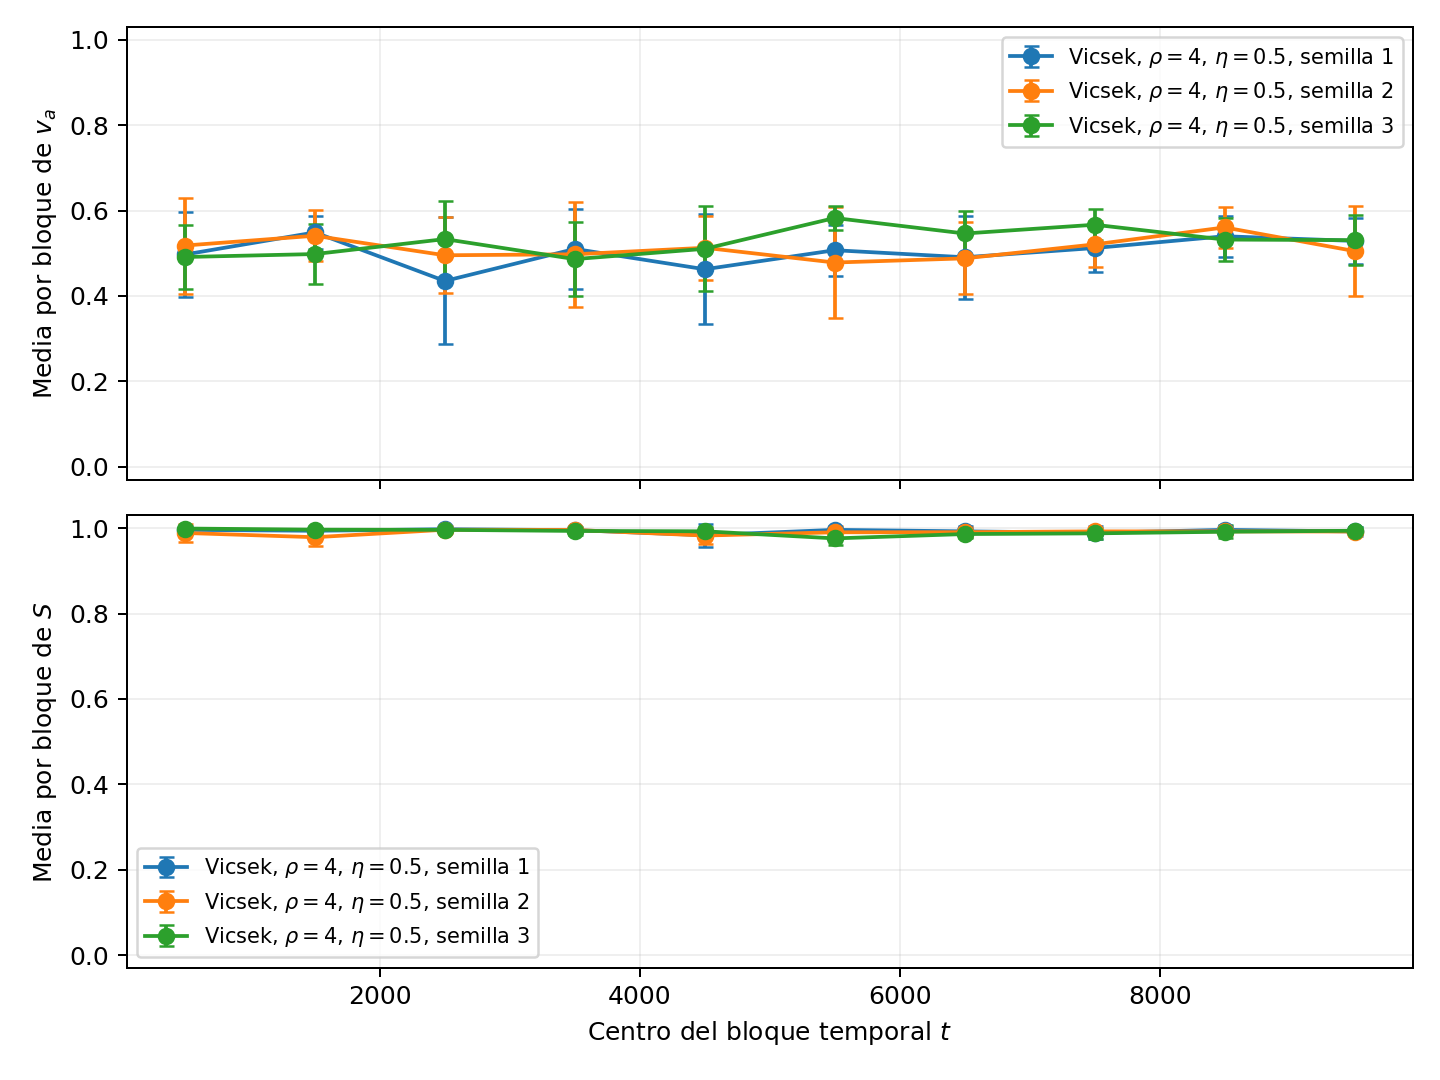
\includegraphics[width=0.86\textwidth]{figuras/bloques-vicsek.png}
\caption{Medias por bloques de \num{1000} unidades de tiempo para el modelo de
Vicsek con $\rho = 4$ y $\eta = 0{,}5$, en tres realizaciones independientes. Las
barras indican la desviación estándar dentro de cada bloque. El primer bloque
contiene el transitorio; a partir de $t = \num{1000}$ las medias fluctúan sin
deriva sistemática.}
\label{fig:bloques}
\end{figure}

Se adoptó $t_0 = \num{4000}$ para todas las corridas. Esta elección conservadora
deja \num{6000} unidades de tiempo para promediar y aplica el mismo criterio a
todas las combinaciones de modelo, densidad y ruido.

\subsection{Promedios y barras de error}

Cada punto de las curvas de la Sección~\ref{sec:resultados} se obtuvo en dos
etapas. Primero se promedió el observable sobre el intervalo estacionario
$[t_0, T]$ dentro de cada semilla, lo que produce diez valores escalares
independientes. Luego se informó la media de esos diez valores y, como barra de
error, su desviación estándar muestral.

El orden de las operaciones es importante. Promediar directamente sobre todas las
muestras temporales de todas las semillas produciría una barra de error
artificialmente pequeña, porque las muestras sucesivas de una misma corrida están
fuertemente correlacionadas y no constituyen observaciones independientes. Al
reducir primero cada corrida a un único número, las diez cantidades que se
comparan sí son estadísticamente independientes entre sí, y su dispersión mide la
variabilidad real del sistema. Este punto es especialmente relevante cerca de la
transición, donde las fluctuaciones son lentas y persisten durante miles de
unidades de tiempo, como se aprecia en la \figref{fig:series-vicsek}.

% =========================== RESULTADOS ===========================
\section{Resultados}
\label{sec:resultados}

\subsection{Dinámica característica}

Las animaciones generadas para cada caso muestran la evolución espacial del
sistema con cada partícula representada por un vector orientado según su
velocidad y coloreado según el ángulo de esa velocidad. La
\figref{fig:cuadros} reúne un cuadro representativo de cuatro de ellas. La
codificación por color permite distinguir de un vistazo el grado de orden: un
sistema polarizado aparece dominado por una única tonalidad, mientras que uno
desordenado presenta todos los colores mezclados.

\begin{figure}[htbp]
\centering
\begin{subfigure}{0.49\textwidth}
  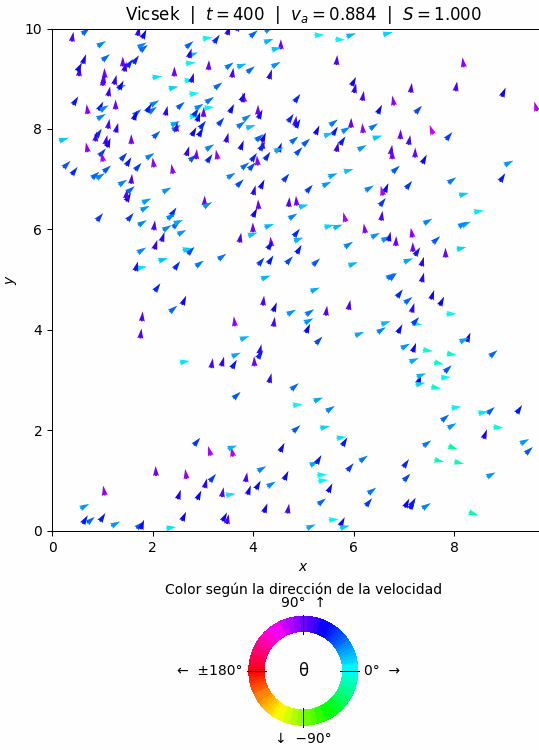
\includegraphics[width=\textwidth]{figuras/cuadro-vicsek-rho4-eta0p25-seed1.png}
  \caption{Vicsek, $\eta = 0{,}25$}
\end{subfigure}
\hfill
\begin{subfigure}{0.49\textwidth}
  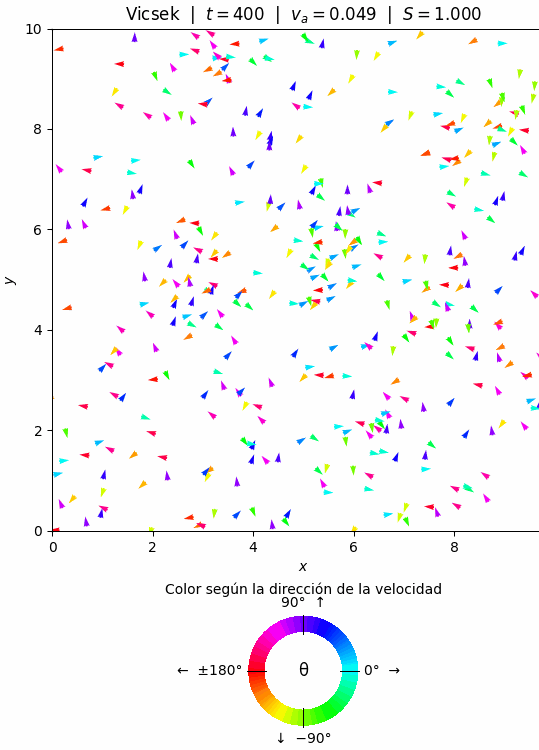
\includegraphics[width=\textwidth]{figuras/cuadro-vicsek-rho4-eta0p75-seed1.png}
  \caption{Vicsek, $\eta = 0{,}75$}
\end{subfigure}

\vspace{0.4cm}
\begin{subfigure}{0.49\textwidth}
  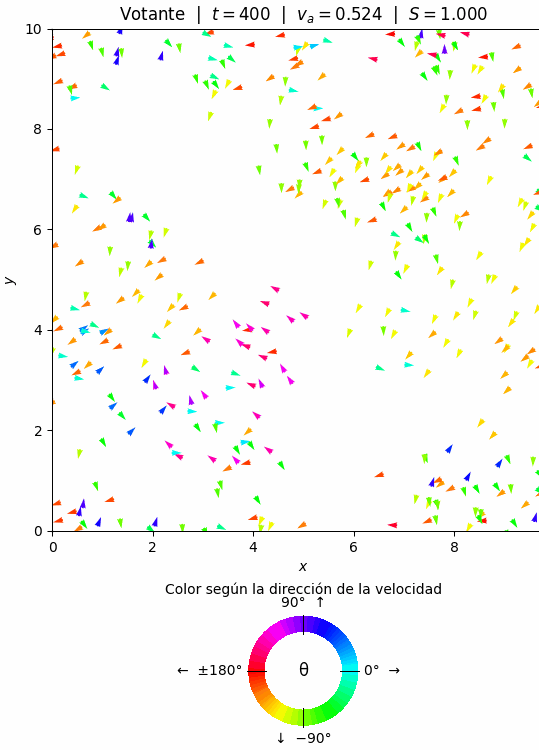
\includegraphics[width=\textwidth]{figuras/cuadro-voter-rho4-eta0p05-seed1.png}
  \caption{Votante, $\eta = 0{,}05$}
\end{subfigure}
\hfill
\begin{subfigure}{0.49\textwidth}
  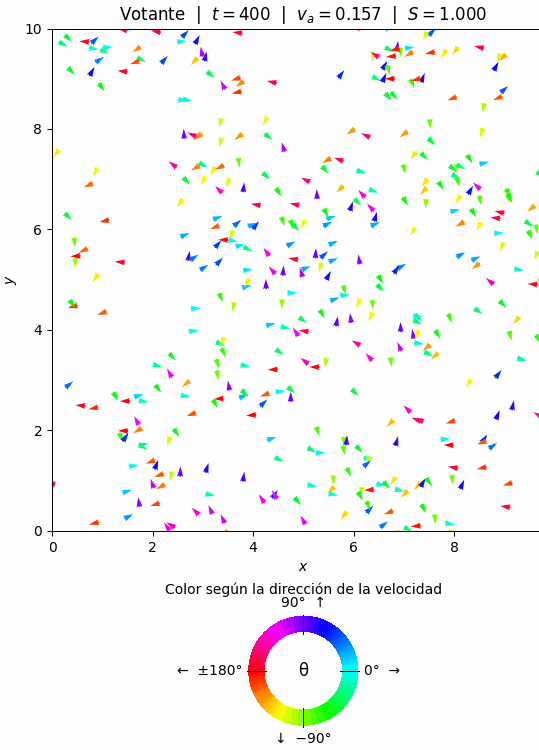
\includegraphics[width=\textwidth]{figuras/cuadro-voter-rho4-eta0p25-seed1.png}
  \caption{Votante, $\eta = 0{,}25$}
\end{subfigure}
\caption{Cuadro final ($t = 400$) de las animaciones características, todas con
$\rho = 4$ y semilla 1. Cada partícula se dibuja como un vector con origen en su
posición, orientado según su velocidad y coloreado según el ángulo de esta,
conforme a la rueda de color incluida en cada cuadro. Los valores instantáneos de
ambos observables figuran en el encabezado. Nótese que el votante ya está
desordenado con $\eta = 0{,}25$ ($v_a = 0{,}157$), ruido con el que Vicsek
conserva $v_a = 0{,}884$.}
\label{fig:cuadros}
\end{figure}

El contraste entre los paneles (a) y (d) resume el resultado central del trabajo:
con el mismo ruido $\eta = 0{,}25$ y la misma densidad, el modelo de Vicsek se
mantiene fuertemente polarizado mientras que el del votante es indistinguible de
un gas desordenado.

\FloatBarrier
\subsection{Evolución temporal de los observables}

La \figref{fig:series-vicsek} muestra la evolución de ambos observables para tres
niveles de ruido representativos. El caso $\eta = 0$ alcanza $v_a = 1$ en unas
pocas decenas de pasos y permanece allí exactamente, como corresponde a una
dinámica sin ruido en la que el alineamiento es absorbente; este comportamiento
funciona como control de la implementación. El caso $\eta = 1$ fluctúa alrededor
de un valor pequeño y constante. El caso intermedio $\eta = 0{,}5$ es el más
informativo: presenta excursiones amplias y lentas, con caídas ocasionales de
$v_a$ desde $0{,}6$ hasta menos de $0{,}2$ que se extienden por centenares de
unidades de tiempo. Son precisamente estas fluctuaciones lentas las que obligan a
promediar sobre intervalos largos y a estimar el error entre realizaciones
independientes.

\begin{figure}[htbp]
\centering
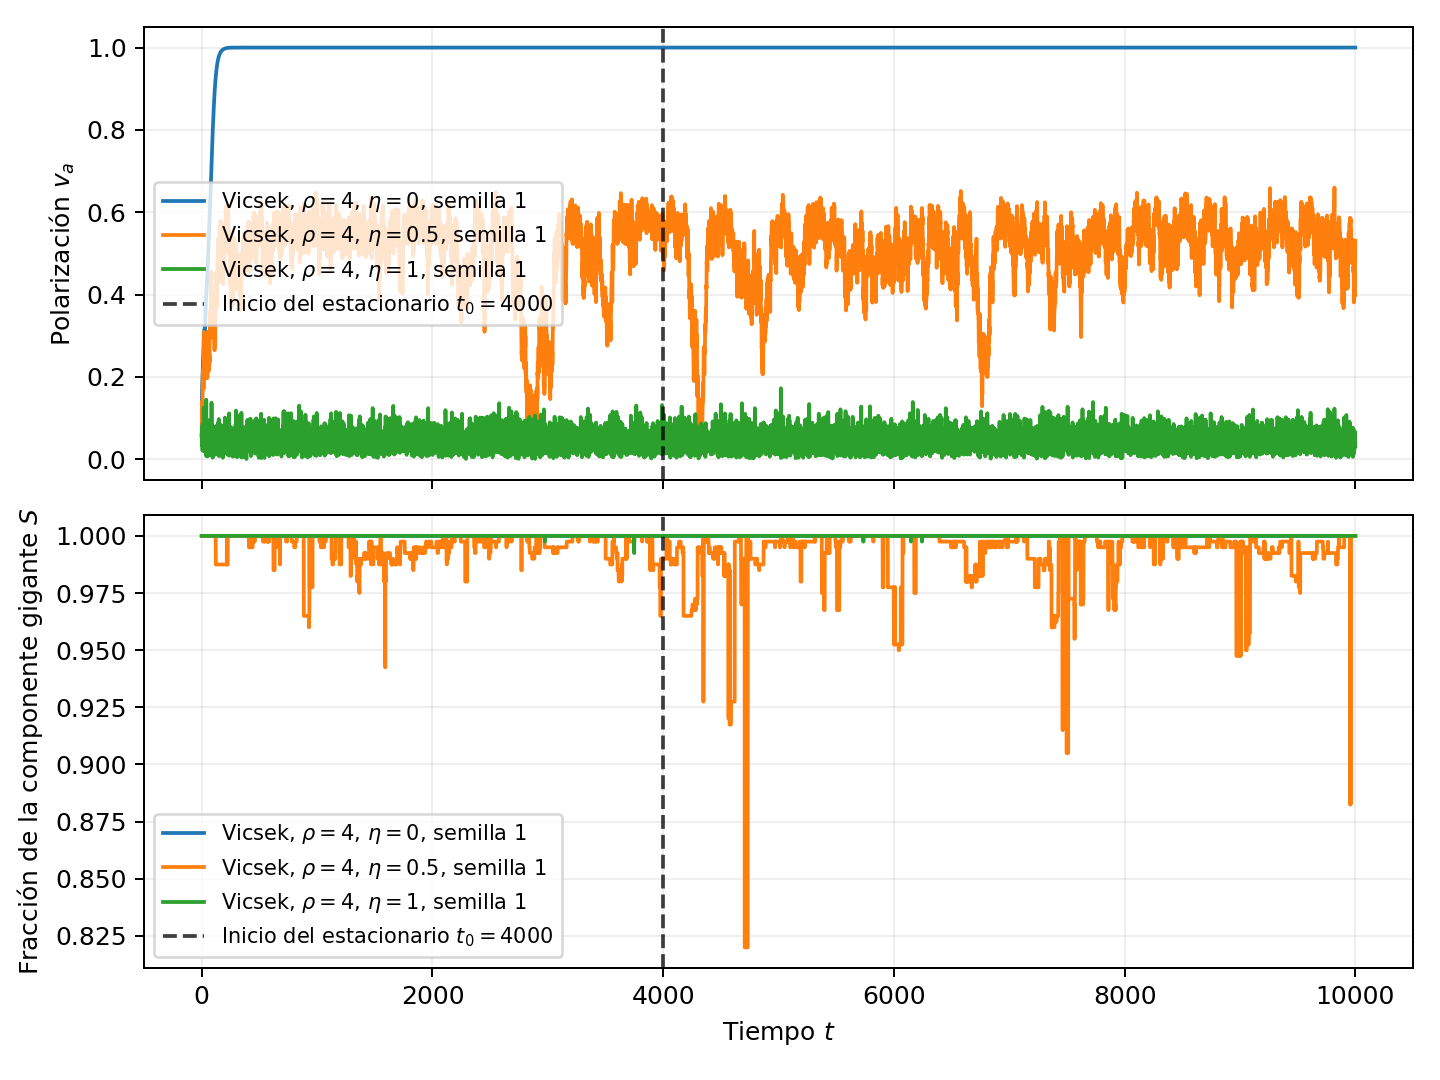
\includegraphics[width=0.88\textwidth]{figuras/series-vicsek.png}
\caption{Evolución temporal de $v_a$ (arriba) y $S$ (abajo) para el modelo de
Vicsek con $\rho = 4$ y semilla 1, en tres niveles de ruido. La línea vertical a
trazos marca el inicio del intervalo de promediado, $t_0 = \num{4000}$. En
$\eta = 0{,}5$ se observan excursiones lentas de gran amplitud.}
\label{fig:series-vicsek}
\end{figure}

El panel inferior revela que, en las densidades pedidas, $S$ permanece por encima
de $0{,}88$ en todo momento y vale prácticamente $1$ salvo en caídas breves. El
sistema está percolado casi siempre, de manera que el desorden direccional
convive con una red de interacción completamente conectada. La
\figref{fig:series-votante} muestra el comportamiento equivalente para el modelo
del votante, con la escala de ruido reducida para cubrir su propio rango de
interés.

\begin{figure}[htbp]
\centering
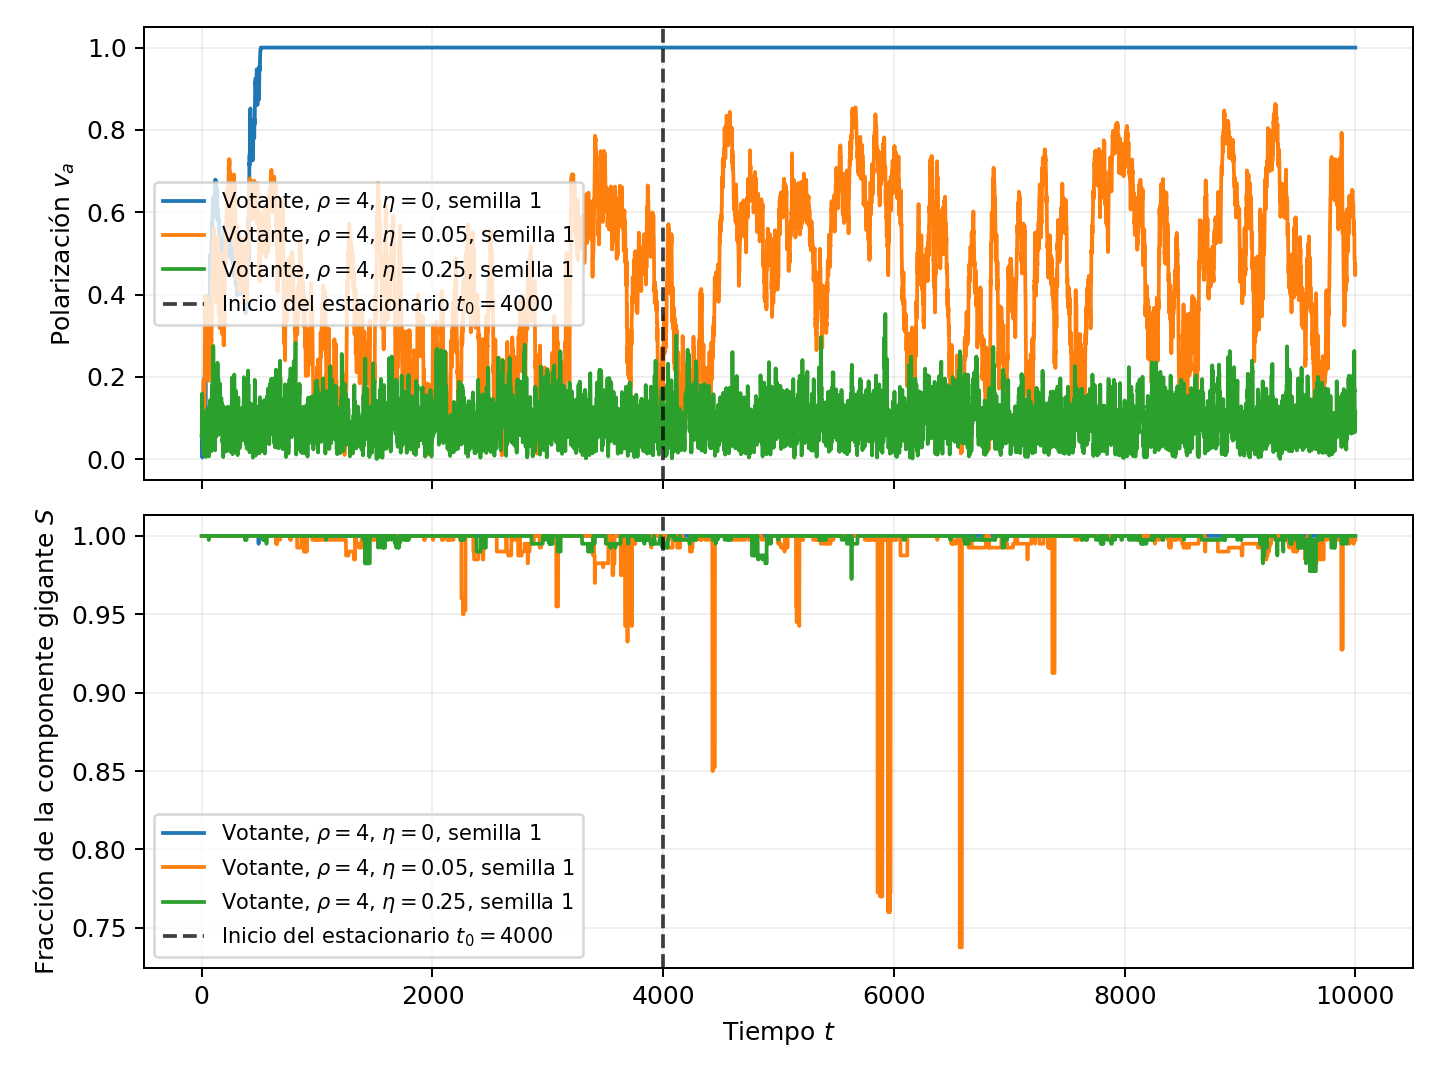
\includegraphics[width=0.88\textwidth]{figuras/series-votante.png}
\caption{Evolución temporal de $v_a$ y $S$ para el modelo del votante con
$\rho = 4$ y semilla 1. Obsérvese que la escala de ruido difiere de la de la
\figref{fig:series-vicsek}: con $\eta = 0{,}25$ el votante ya está desordenado.
La línea vertical marca $t_0 = \num{4000}$.}
\label{fig:series-votante}
\end{figure}

\FloatBarrier
\subsection{Polarización en función del ruido}

La \figref{fig:va-eta} reúne las seis curvas de polarización estacionaria. La
diferencia entre modelos es de casi un orden de magnitud en la escala de ruido.
Para cuantificarla se define $\eta_{1/2}$ como el ruido al que $v_a$ desciende
hasta $0{,}5$, obtenido por interpolación lineal entre los puntos medidos; los
valores se listan en la \tabref{tab:eta-medio}.

\begin{figure}[htbp]
\centering
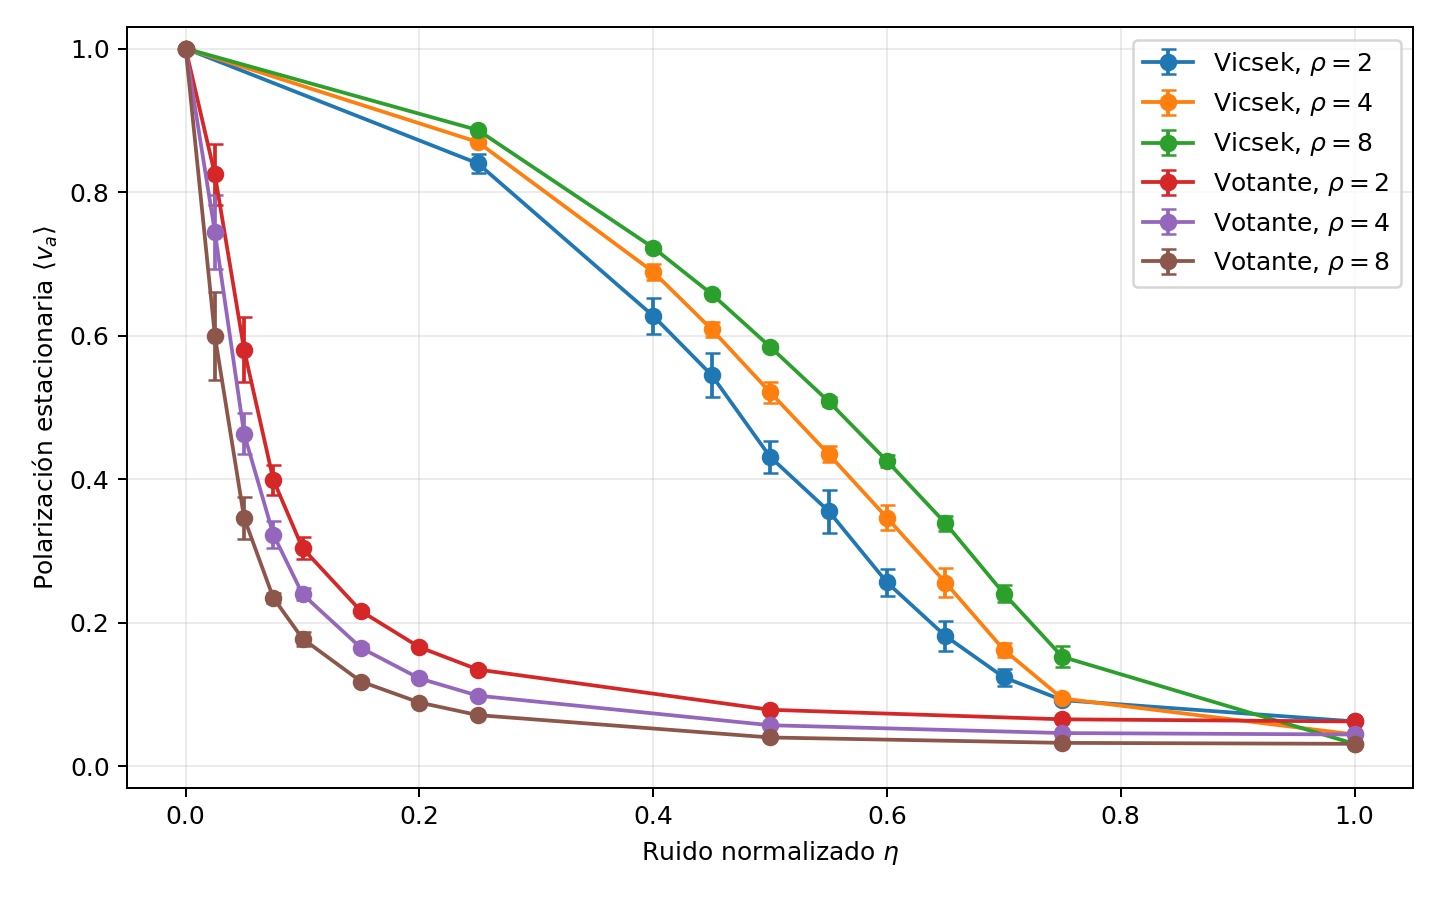
\includegraphics[width=0.88\textwidth]{figuras/va-vs-eta.png}
\caption{Polarización estacionaria en función del ruido para ambos modelos y las
tres densidades. Cada punto es el promedio sobre \num{10} realizaciones
independientes de la media temporal en $[\num{4000}, \num{10000}]$; las barras
son la desviación estándar entre realizaciones. Las mallas de $\eta$ difieren
entre modelos para resolver cada transición.}
\label{fig:va-eta}
\end{figure}

\begin{table}[htbp]
\centering
\caption{Ruido $\eta_{1/2}$ al que la polarización cae a $0{,}5$, y su
equivalente en la escala del trabajo original según la \ecref{eq:conversion}. La
última columna muestra cuántas veces más ruido tolera Vicsek que el votante a
igual densidad.}
\label{tab:eta-medio}
\begin{tabular}{lccc}
\toprule
$\rho$ & $\eta_{1/2}$ (Vicsek) & $\eta_{1/2}$ (votante) & Cociente \\
\midrule
2 & 0,470 & 0,061 & 7,7 \\
4 & 0,512 & 0,047 & 11,0 \\
8 & 0,555 & 0,035 & 15,9 \\
\bottomrule
\end{tabular}
\end{table}

Las dos familias de curvas no solo difieren en escala, sino que responden a la
densidad en sentidos opuestos. En el modelo de Vicsek, aumentar la densidad
\emph{favorece} el orden: a $\eta = 0{,}25$ la polarización crece de
$0{,}840 \pm 0{,}013$ a $0{,}886 \pm 0{,}002$ al pasar de $\rho = 2$ a
$\rho = 8$, y $\eta_{1/2}$ se desplaza de $0{,}470$ a $0{,}555$. En el modelo del
votante ocurre lo contrario: a $\eta = 0{,}025$ la polarización \emph{cae} de
$0{,}825 \pm 0{,}042$ a $0{,}600 \pm 0{,}062$ en el mismo rango de densidades, y
$\eta_{1/2}$ disminuye de $0{,}061$ a $0{,}035$.

Esta inversión se explica por la naturaleza estadística de cada regla. En Vicsek,
el promedio de la \ecref{eq:vicsek} se toma sobre $|\mathcal{N}_i|$ direcciones,
y el error de ese promedio decrece con la raíz del número de vecinas: más
densidad implica un promedio más confiable y, por lo tanto, mayor resistencia al
ruido. En el votante, la \ecref{eq:votante} usa una sola vecina cualquiera sea la
densidad, de modo que la calidad de la información copiada no mejora al haber más
vecinas. Lo único que cambia al aumentar la densidad es que la red de interacción
tiene más nodos entre los que debe propagarse el consenso, y el ruido dispone de
más oportunidades por unidad de tiempo para destruirlo antes de que se propague.
El resultado neto es que la densidad perjudica al orden en el modelo del votante.

La misma asimetría se manifiesta en el transitorio. En $\eta = 0$ el modelo del
votante tarda tanto más en alcanzar $v_a = 1$ cuanto mayor es la densidad
—alrededor de $t = \num{1500}$ para $\rho = 2$ y de $t = \num{3000}$ para
$\rho = 8$—, mientras que Vicsek converge en unas pocas decenas de pasos con
independencia de la densidad. Es el mismo mecanismo visto en el tiempo: el
consenso por copia debe propagarse nodo a nodo, y ese proceso se vuelve más lento
al crecer el sistema.

Conviene señalar que el sistema de $\rho = 4$ coincide con uno de los estudiados
en el trabajo original ($N = 400$, $L = 10$)~\cite{vicsek1995}. Expresado en la
escala de aquella referencia mediante la \ecref{eq:conversion}, el valor
$\eta_{1/2} = 0{,}512$ equivale a $\eta_V = 3{,}22$, del orden de magnitud
esperado para un sistema de este tamaño.

Un último aspecto de la \figref{fig:va-eta} merece atención. En $\eta = 1$ las
curvas no se anulan exactamente porque la suma de un número finito de direcciones
aleatorias presenta fluctuaciones. Para $N$ direcciones independientes y
uniformes, su módulo sigue una distribución de Rayleigh y el valor residual es
del orden de
\[
\langle v_a \rangle \simeq \frac{\sqrt{\pi}}{2\sqrt{N}}.
\]
Por lo tanto, una polarización pequeña en este límite es compatible con un estado
completamente desordenado y no debe interpretarse como orden residual.

\subsection{Componente gigante}

La \figref{fig:series-densidades} muestra la evolución temporal de la componente
gigante en las tres densidades pedidas, a ruido intermedio. El comportamiento
depende fuertemente de $\rho$: con $\rho = 8$ la red permanece completamente
conectada en todo momento ($S \ge 0{,}985$), con $\rho = 4$ aparecen caídas
esporádicas que no bajan de $0{,}82$, y con $\rho = 2$ la fragmentación es
frecuente y llega a reducir la componente mayor hasta $0{,}44$. Los promedios
estacionarios correspondientes son $0{,}926$, $0{,}992$ y $0{,}9995$.

\begin{figure}[htbp]
\centering
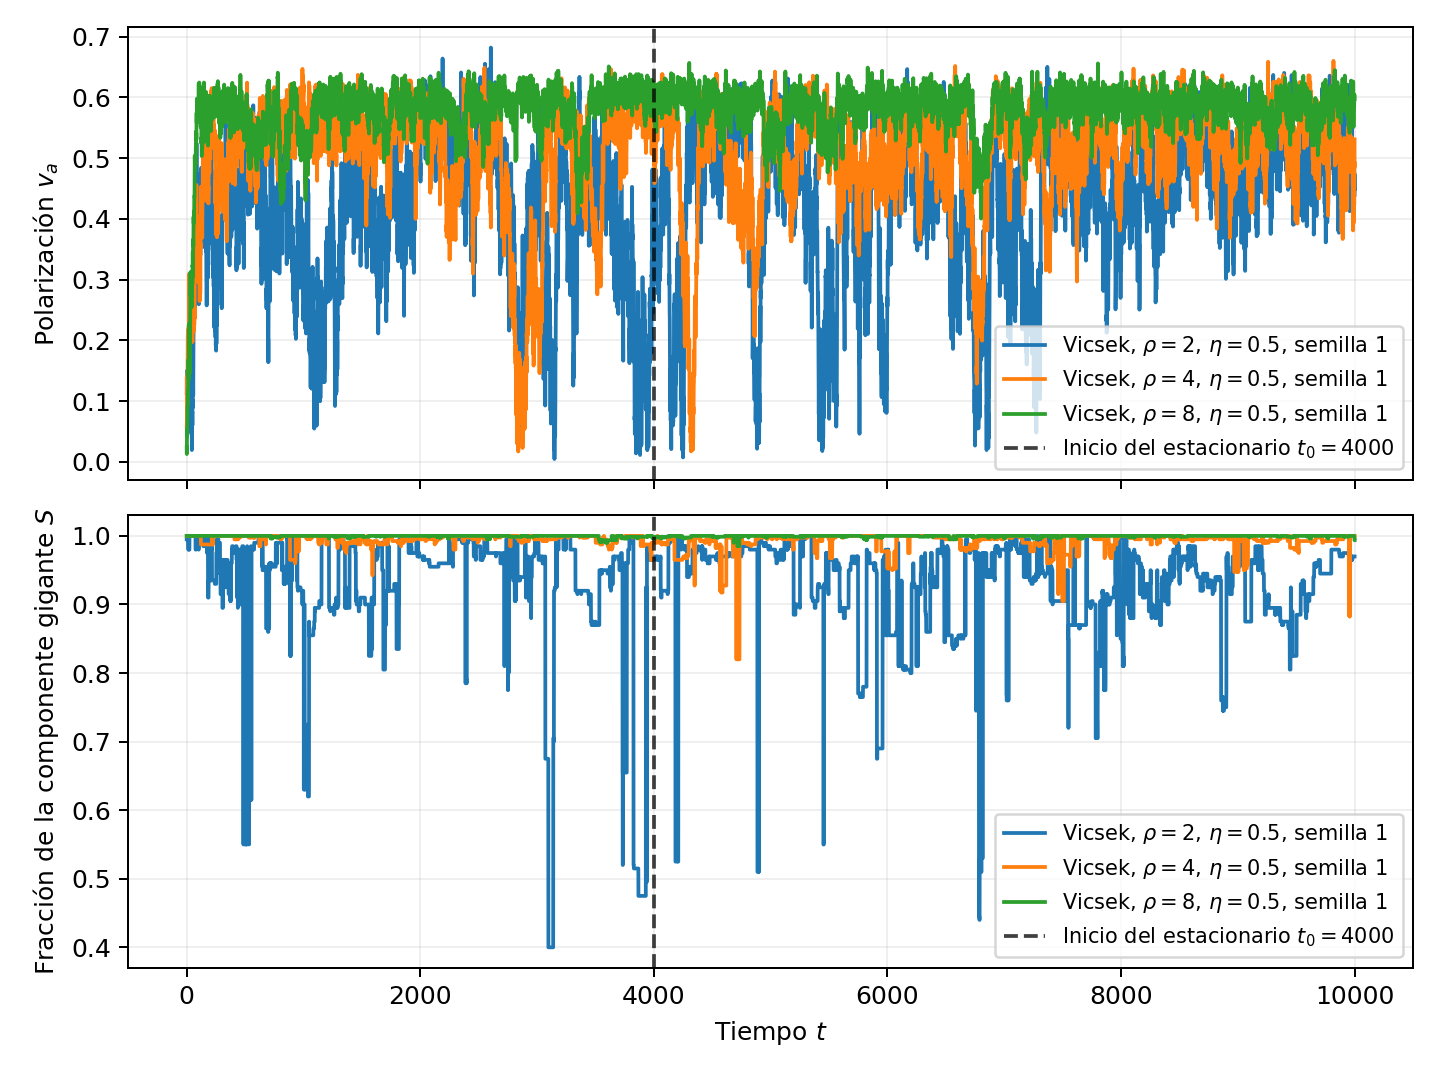
\includegraphics[width=0.88\textwidth]{figuras/series-densidades.png}
\caption{Evolución temporal de $v_a$ y $S$ para el modelo de Vicsek con
$\eta = 0{,}5$ y semilla 1, en las tres densidades pedidas. La línea vertical
marca $t_0 = \num{4000}$. Las caídas de $S$ en $\rho = 2$ coinciden
temporalmente con caídas de $v_a$.}
\label{fig:series-densidades}
\end{figure}

Un rasgo relevante de la \figref{fig:series-densidades} es que las caídas de $S$
en $\rho = 2$ ocurren simultáneamente con caídas de $v_a$. La fragmentación de la
red y la pérdida de alineamiento no son fenómenos independientes: cuando el grupo
se parte, los fragmentos evolucionan sin intercambiar información y sus
direcciones divergen, lo que reduce la polarización global. Esta correlación
temporal anticipa la relación entre ambos observables que se analiza en la
Sección~\ref{sec:va-s}.

Aun así, en las tres densidades pedidas el observable $S$ resulta poco
informativo como parámetro escalar. Como muestra la \figref{fig:s-eta}, permanece por encima de $0{,}90$ en todo el rango
de ruido y, para $\rho = 8$, es indistinguible de $1$ dentro del error. La razón
es geométrica: con $r_c = 1$ y $\rho \ge 2$ cada partícula tiene en promedio
$\pi r_c^2 \rho \ge 6{,}3$ vecinas, muy por encima del umbral de percolación, de
modo que la red de interacción forma una única componente conexa
independientemente de cómo estén orientadas las velocidades.

\begin{figure}[htbp]
\centering
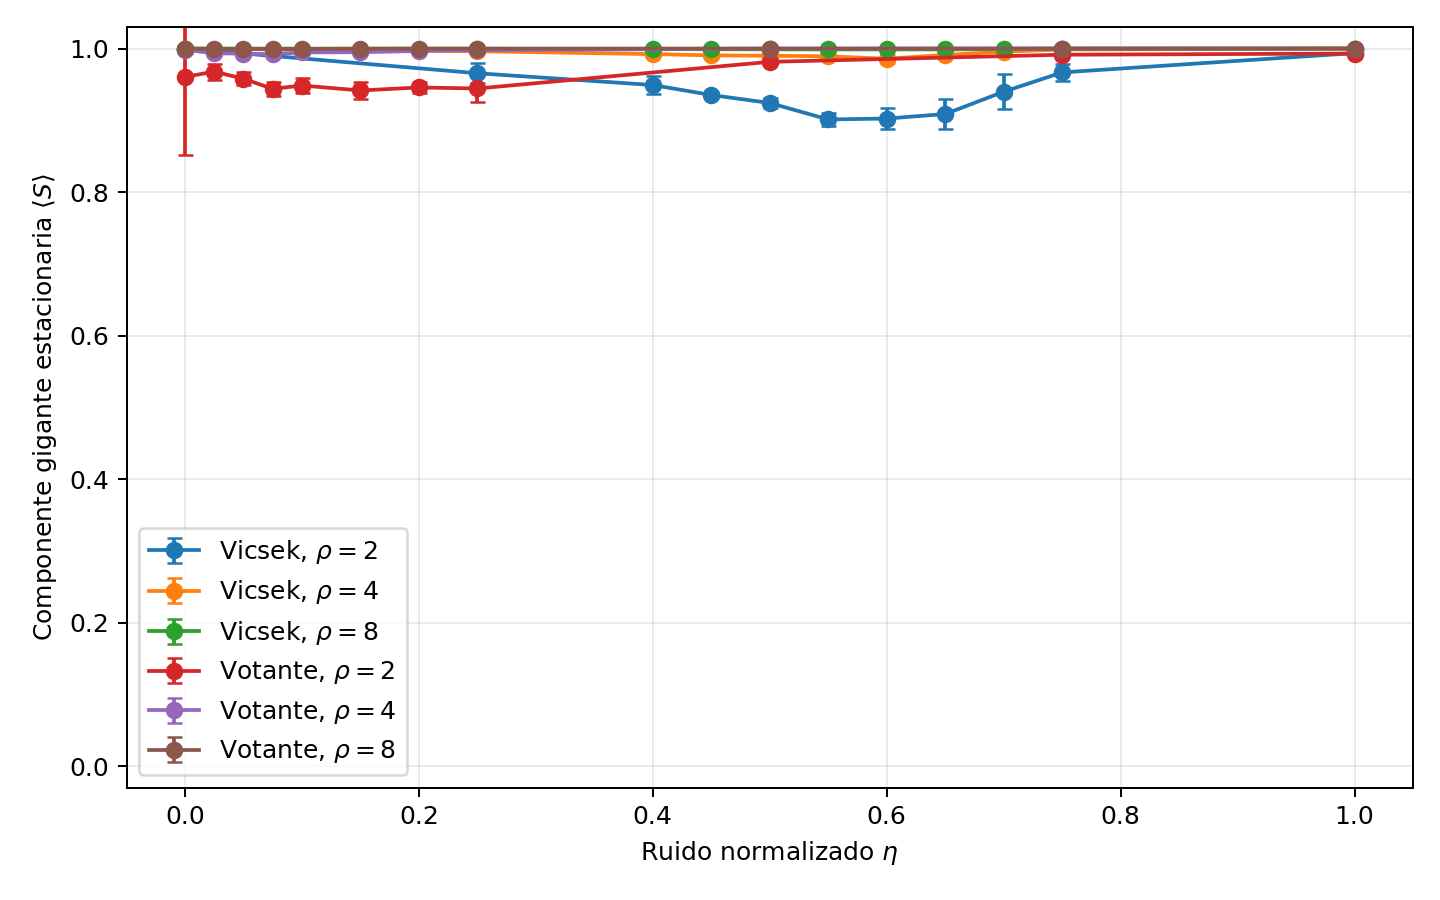
\includegraphics[width=0.88\textwidth]{figuras/s-vs-eta.png}
\caption{Fracción de partículas en la componente gigante para las densidades
pedidas. El observable satura cerca de $1$ en todo el rango de ruido, con un
mínimo poco profundo alrededor de $\eta \approx 0{,}6$ para $\rho = 2$.}
\label{fig:s-eta}
\end{figure}

El único rasgo apreciable es un mínimo poco profundo en $\rho = 2$, donde $S$
desciende hasta $0{,}90$ alrededor de $\eta \approx 0{,}6$ y vuelve a crecer
hasta $0{,}99$ en $\eta = 1$. El comportamiento no monótono tiene sentido físico:
con ruido nulo las partículas se mueven en paralelo y conservan la configuración
espacial inicial, que está percolada; con ruido máximo el movimiento es
difusivo y la distribución permanece homogénea, también percolada; en el ruido
intermedio, en cambio, la formación de grupos que se desplazan coherentemente
deja regiones vacías entre ellos y fragmenta ocasionalmente la red.

Para que el observable resulte discriminante se recurrió a las densidades bajas
descritas en la Sección~\ref{sec:simulaciones}. La \figref{fig:s-eta-baja}
muestra que allí $S$ sí recorre casi todo su rango: cae desde valores próximos a
$0{,}95$ en $\eta = 0$ hasta $0{,}15$--$0{,}20$ en $\eta = 1$.

\begin{figure}[htbp]
\centering
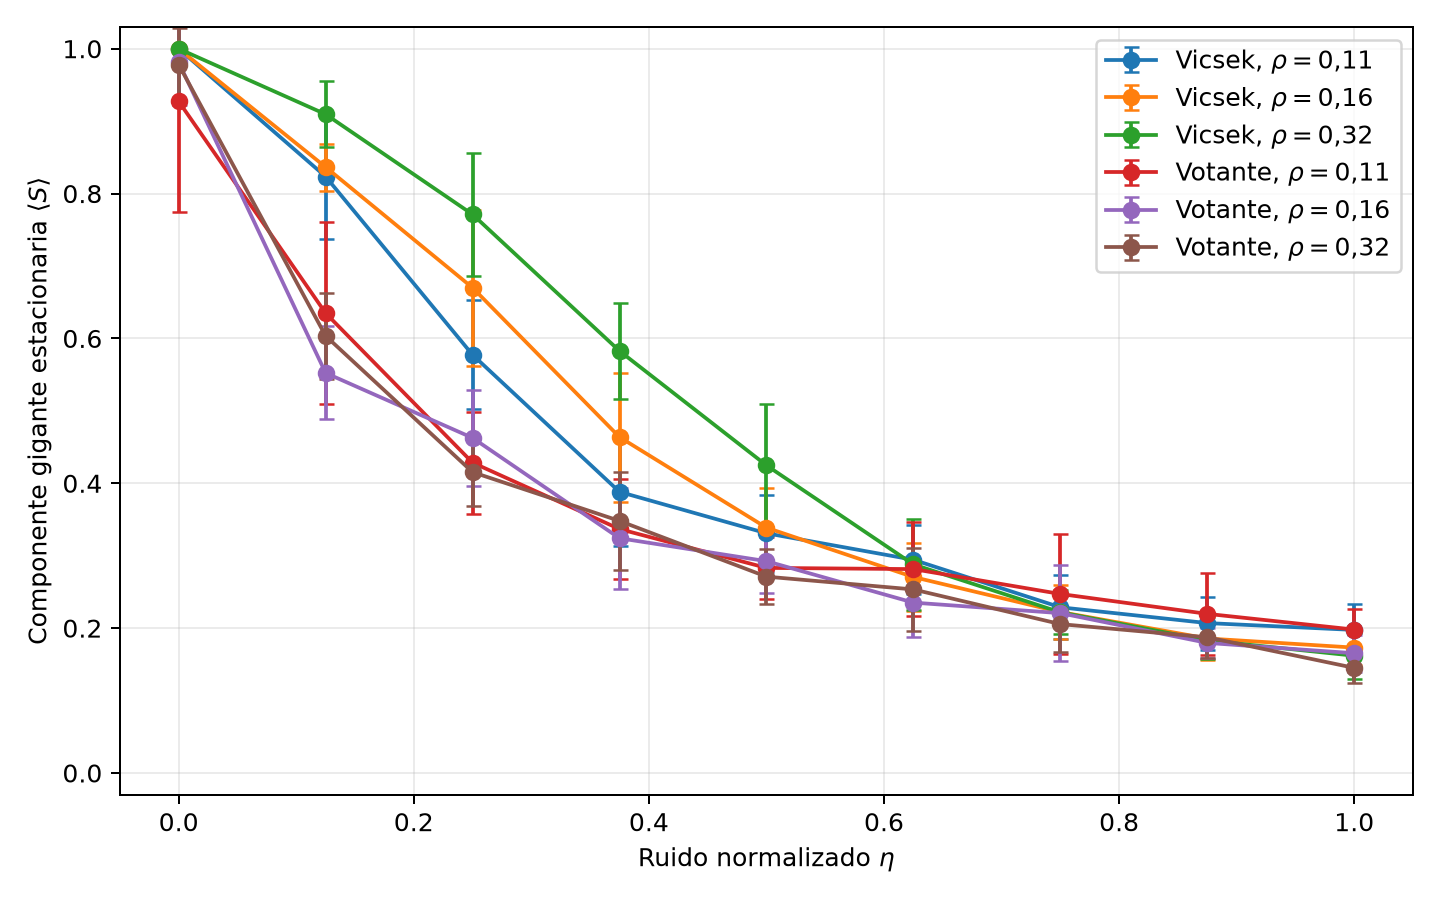
\includegraphics[width=0.88\textwidth]{figuras/s-vs-eta-baja-densidad.png}
\caption{Componente gigante en función del ruido para las densidades nominales
$1/\pi$, $1/(2\pi)$ y $1/(3\pi)$, que con $L = 10$ corresponden a $N = 32$, $16$
y $11$ partículas. A diferencia de la \figref{fig:s-eta}, aquí el observable
recorre casi todo su rango y separa claramente ambos modelos.}
\label{fig:s-eta-baja}
\end{figure}

\begin{figure}[htbp]
\centering
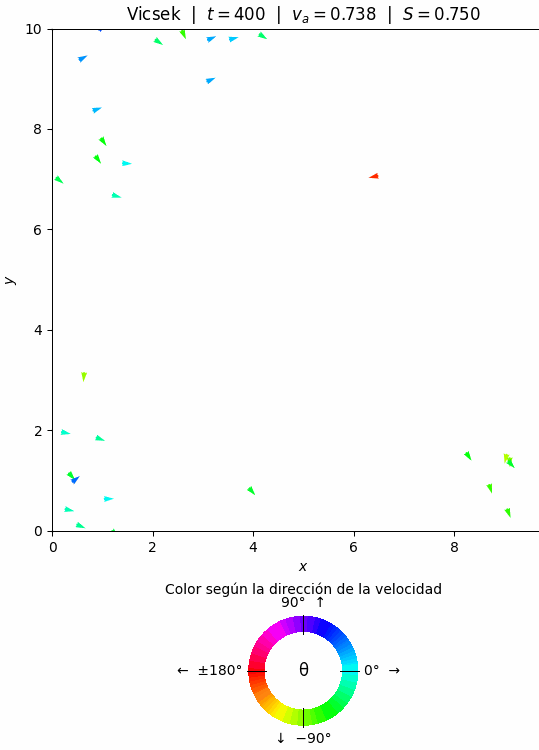
\includegraphics[width=0.46\textwidth]{figuras/cuadro-vicsek-rho0p32-eta0p25-seed1.png}
\caption{Cuadro final ($t = 400$) de la animación característica en densidad
baja: Vicsek con $\rho \simeq 1/\pi$ ($N = 32$) y $\eta = 0{,}25$. A diferencia
de la \figref{fig:cuadros}, aquí las partículas forman grupos separados por
regiones vacías y la red de interacción deja de estar percolada
($S = 0{,}750$ en este cuadro).}
\label{fig:cuadro-baja}
\end{figure}

El cambio de régimen es visible directamente en la dinámica. La
\figref{fig:cuadro-baja} muestra que, en densidad baja, las partículas se
organizan en grupos separados por regiones vacías, en contraste con la ocupación
homogénea de la \figref{fig:cuadros}.

En este régimen reaparece la jerarquía entre modelos: a igual densidad y ruido,
el votante presenta sistemáticamente menor $S$ que Vicsek en la región
$\eta \lesssim 0{,}5$. Con $\rho \simeq 1/\pi$ y $\eta = 0{,}25$, por ejemplo, se
obtiene $S = 0{,}771$ para Vicsek y $S = 0{,}415$ para el votante. La
interpretación es directa: mantener el grupo espacialmente cohesionado requiere
que las partículas se muevan en direcciones parecidas, y como el votante pierde
antes el orden direccional, también pierde antes la cohesión. Para
$\eta \gtrsim 0{,}6$ las seis curvas colapsan, porque con ruido alto ningún
modelo sostiene agrupamiento y $S$ queda determinado únicamente por las
fluctuaciones de una distribución espacial esencialmente aleatoria.

\FloatBarrier
\subsection{Relación entre polarización y componente gigante}
\label{sec:va-s}

La \figref{fig:va-s} representa $v_a$ frente a $S$ recorriendo $\eta$ como
parámetro implícito. En las densidades pedidas los puntos se acumulan sobre el
borde derecho del gráfico, ya que $S$ apenas varía mientras $v_a$ recorre todo su
rango: en un sistema percolado la polarización no está limitada por la
conectividad, y ambos observables resultan prácticamente independientes.

\begin{figure}[htbp]
\centering
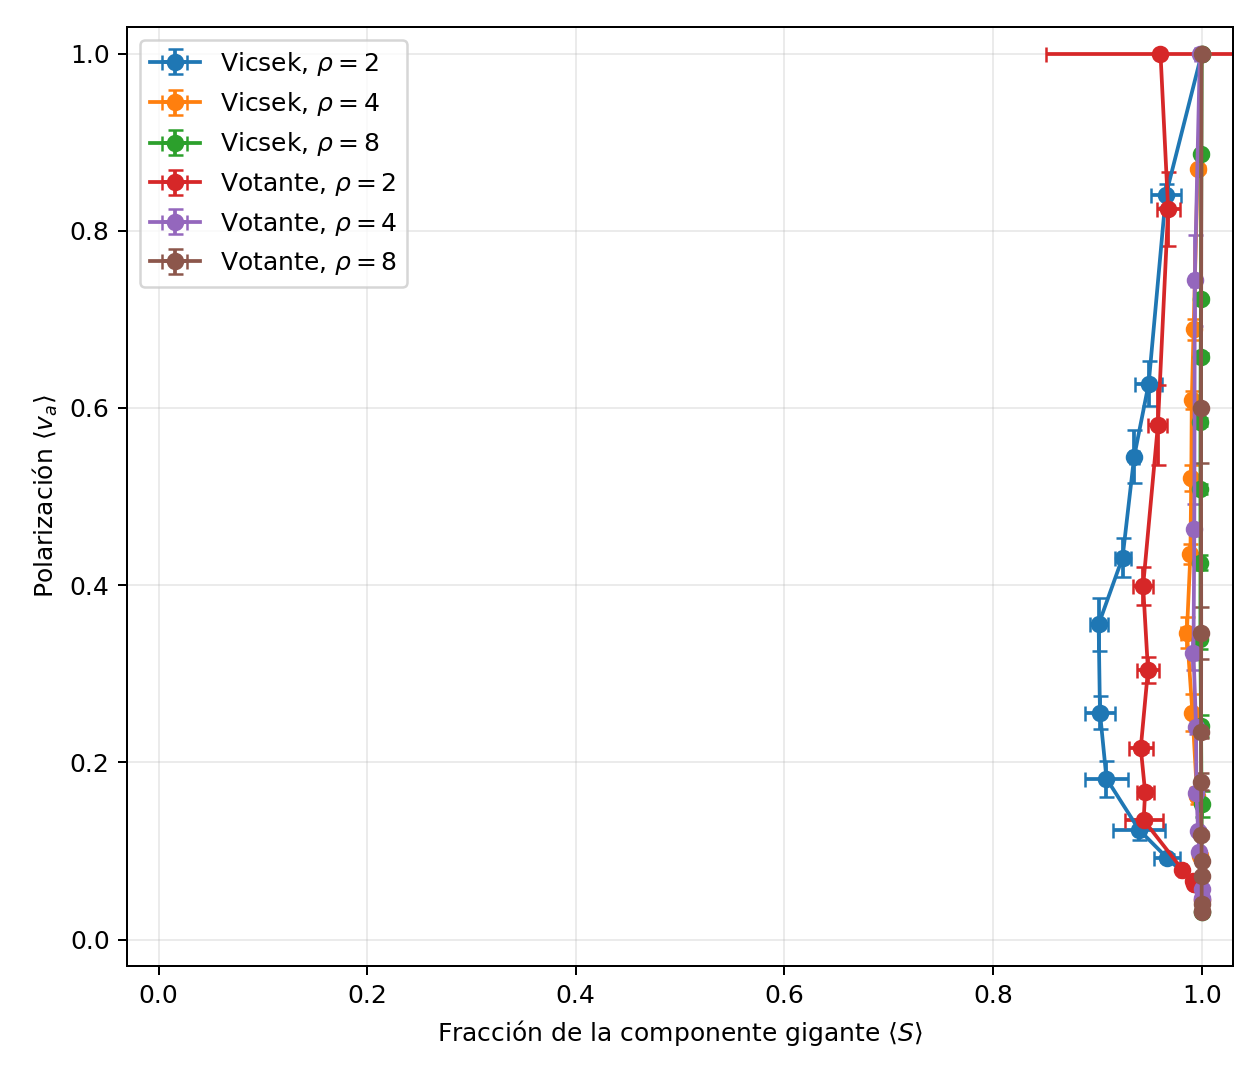
\includegraphics[width=0.72\textwidth]{figuras/va-vs-s.png}
\caption{Polarización estacionaria frente a la componente gigante en las
densidades pedidas, con $\eta$ como parámetro implícito a lo largo de cada curva.
La escasa variación horizontal indica que en este régimen la conectividad no
limita la polarización.}
\label{fig:va-s}
\end{figure}

La \figref{fig:va-s} muestra que, para las densidades pedidas, la escasa variación
de $S$ concentra los puntos cerca del borde derecho y dificulta observar una
relación entre ambos observables. Por eso conviene repetir el análisis en las
densidades bajas. Antes, la \figref{fig:va-eta-baja} presenta $v_a$ frente a
$\eta$ en ese régimen. Se conserva la jerarquía entre modelos, pero el rasgo
dominante es que el piso de ruido máximo es mucho más alto que en la
\figref{fig:va-eta}, porque aquí el número de partículas es menor. En estos
sistemas pequeños, una polarización de $0{,}25$ puede ser compatible con el
desorden y las curvas deben interpretarse teniendo en cuenta ese efecto de tamaño
finito.

\begin{figure}[htbp]
\centering
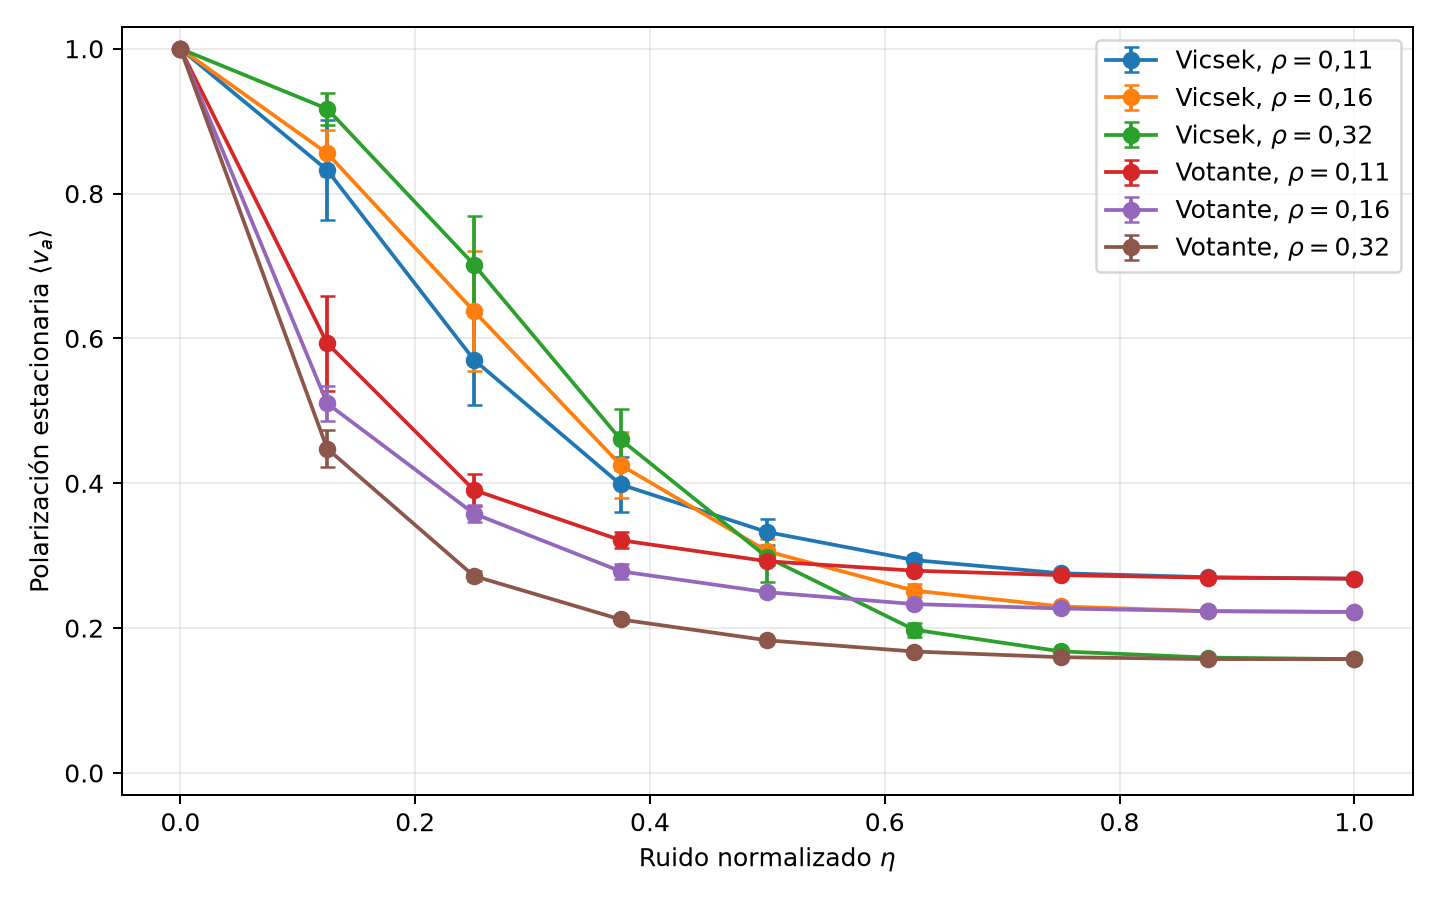
\includegraphics[width=0.88\textwidth]{figuras/va-vs-eta-baja-densidad.png}
\caption{Polarización estacionaria en función del ruido en las densidades bajas.
El valor residual en $\eta = 1$ es un efecto de tamaño finito y crece al
disminuir $N$.}
\label{fig:va-eta-baja}
\end{figure}

El panorama cambia en densidad baja. La \figref{fig:va-s-baja}, con $v_a$ en el
eje horizontal y $S$ en el vertical, muestra que los puntos se ordenan a lo largo
de una relación monótona y aproximadamente lineal compartida por las seis series:
la componente gigante crece con la polarización. La correspondencia es
notablemente estrecha —para $\rho \simeq 1/(3\pi)$ se obtienen los pares
$(v_a,S)$ iguales a $(0{,}571;\,0{,}577)$ y $(0{,}398;\,0{,}388)$,
prácticamente sobre la diagonal—.

\begin{figure}[htbp]
\centering
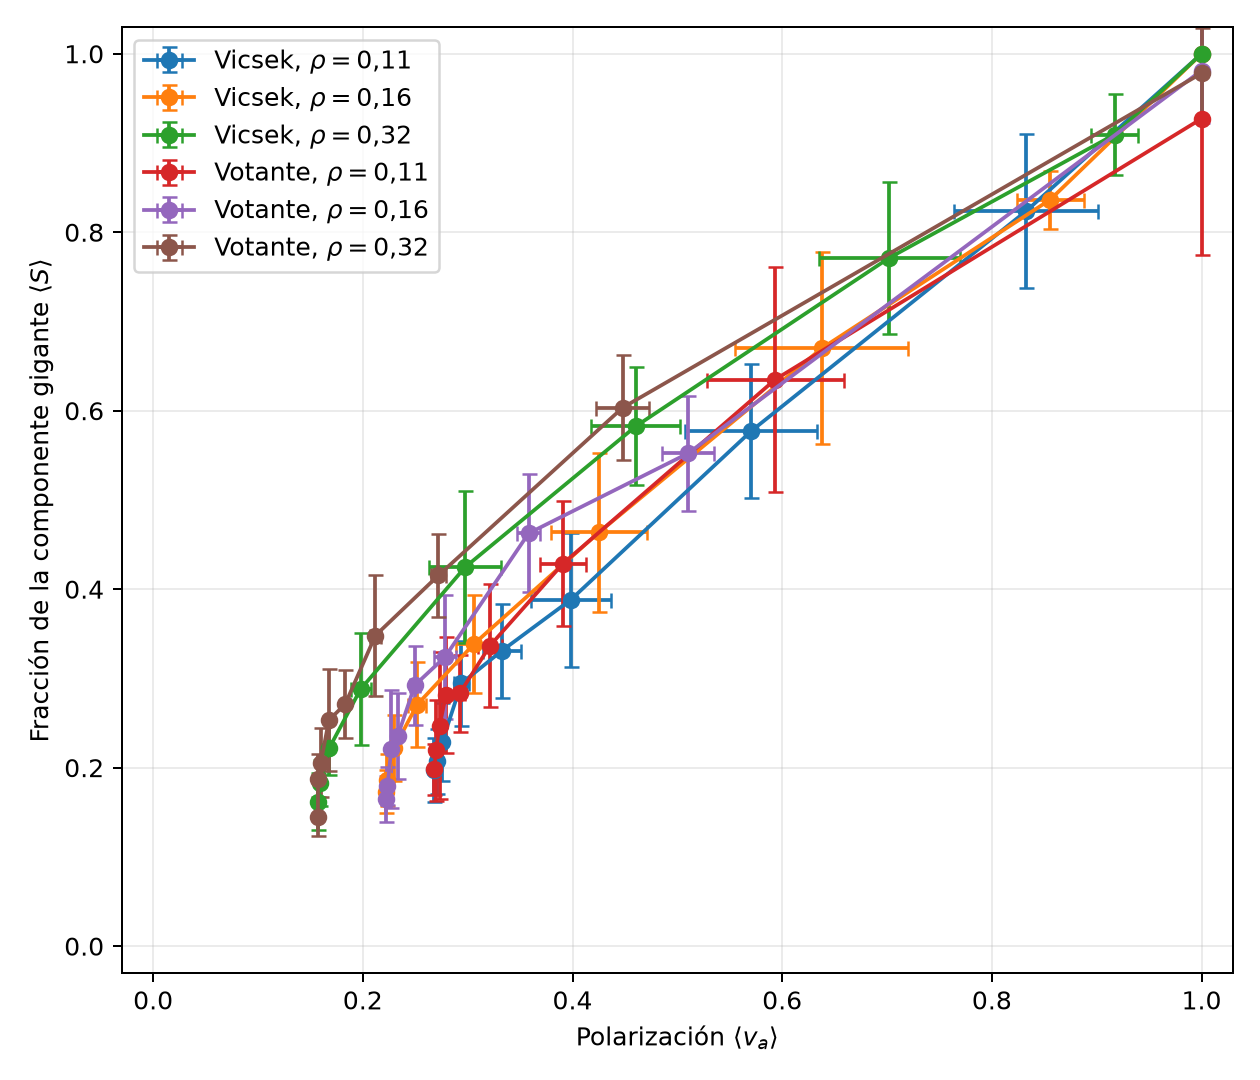
\includegraphics[width=0.72\textwidth]{figuras/va-vs-s-baja-densidad.png}
\caption{Componente gigante frente a polarización en las densidades bajas. Las
seis series colapsan aproximadamente sobre una misma relación monótona, lo que
indica que en este régimen la conectividad y el orden direccional están
estrechamente relacionados.}
\label{fig:va-s-baja}
\end{figure}

La lectura conjunta de ambas figuras precisa el papel de cada observable. Cuando
la red está percolada, la información direccional puede recorrer todo el sistema
y el orden queda limitado únicamente por el ruido; $S$ no aporta información
adicional. Cuando la red se fragmenta, cada componente conexa alinea sus
partículas por separado y las distintas componentes lo hacen en direcciones
mutuamente independientes, de modo que la polarización global queda acotada por
el tamaño relativo de la componente mayor. En ese régimen $S$ deja de ser un
observable redundante y pasa a ser el que fija el techo de $v_a$.

\FloatBarrier
\subsection{Desempeño del Cell Index Method}

El tiempo de búsqueda de vecinos se midió por separado en corridas dedicadas
ejecutadas de a una por vez, dado que las mediciones tomadas durante los barridos
de producción —doce procesos simultáneos— resultaron inutilizables por la
competencia entre procesos. La \tabref{tab:cim} resume los resultados y los
compara con los del trabajo práctico anterior sobre configuraciones periódicas.

\begin{table}[htbp]
\centering
\caption{Tiempo medio de búsqueda de vecinos por invocación del CIM. Los valores
del TP1 corresponden a sus configuraciones periódicas con el mismo $N$. La última
columna normaliza el tiempo por evaluación de distancia efectivamente realizada.}
\label{tab:cim}
\begin{tabular}{llrrrrr}
\toprule
Origen & Modelo & $N$ & $\rho$ & $L$ & $t$ [\si{\micro\second}] & $t$/eval. [\si{\nano\second}] \\
\midrule
TP2 & Vicsek  & 200 & 2,00 & 10,0 & 82,9  & 17,9 \\
TP2 & Votante & 200 & 2,00 & 10,0 & 47,7  & 20,3 \\
TP2 & Vicsek  & 400 & 4,00 & 10,0 & 248,5 & 16,9 \\
TP2 & Votante & 400 & 4,00 & 10,0 & 154,5 & 17,0 \\
TP2 & Vicsek  & 800 & 8,00 & 10,0 & 914,9 & 16,3 \\
TP2 & Votante & 800 & 8,00 & 10,0 & 577,7 & 16,0 \\
\midrule
TP1 & ---     & 200 & 1,25 & 12,6 & 95,6  & 34,8 \\
TP1 & ---     & 200 & 0,50 & 20,0 & 45,0  & 43,8 \\
TP1 & ---     & 800 & 1,25 & 25,3 & 406,8 & 37,0 \\
TP1 & ---     & 800 & 2,00 & 20,0 & 582,2 & 34,8 \\
\bottomrule
\end{tabular}
\end{table}

Los tiempos absolutos no son directamente comparables, porque a igual $N$ las
densidades difieren: las configuraciones de este trabajo son entre $1{,}6$ y
$6{,}4$ veces más densas que las del TP1, y el costo del CIM está gobernado por
la cantidad de partículas contenidas en el bloque de nueve celdas, no por $N$. La
comparación adecuada es la de la última columna, que normaliza por el número de
evaluaciones de distancia realmente ejecutadas. En esa métrica la implementación
del TP2 requiere entre \SI{16}{\nano\second} y \SI{20}{\nano\second} por
evaluación, frente a \SI{35}{\nano\second} a \SI{44}{\nano\second} en el TP1: es
aproximadamente el doble de rápida por operación elemental. La diferencia es
atribuible a la geometría del problema, ya que el TP1 trabajaba con discos de
radio finito y debía calcular distancias borde a borde, mientras que aquí las
partículas son puntuales y basta comparar el cuadrado de la distancia con
$r_c^2$, sin extracción de raíz ni corrección por radios.

Un efecto secundario, visible en la \tabref{tab:cim}, es que el modelo influye
sobre el costo de la búsqueda pese a no intervenir en ella: a igual $N$ y $\rho$,
las corridas de Vicsek requieren cerca del doble de evaluaciones de distancia que
las del votante. La causa es que ambas fueron medidas con $\eta = 0{,}5$, ruido
con el que Vicsek se encuentra parcialmente ordenado y forma agrupamientos densos
—que concentran muchas partículas en pocas celdas— mientras que el votante ya
está desordenado y distribuye las partículas de manera casi homogénea. El costo
del CIM depende, entonces, del estado dinámico del sistema y no solo de sus
parámetros nominales.

\begin{figure}[htbp]
\centering
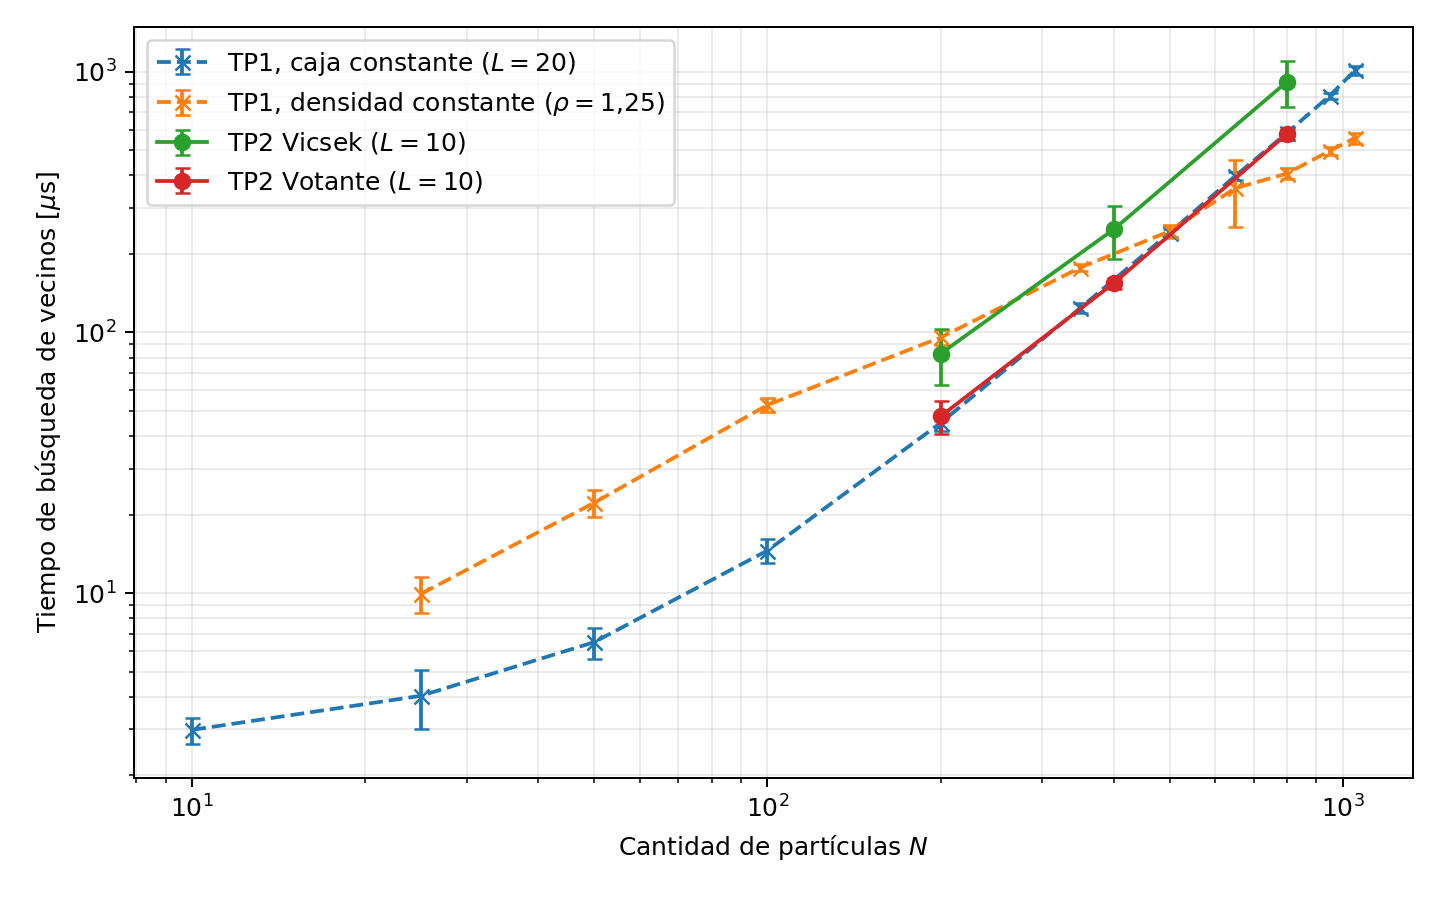
\includegraphics[width=0.88\textwidth]{figuras/cim-comparacion.png}
\caption{Tiempo de búsqueda de vecinos en función de $N$, en escala doblemente
logarítmica. Se comparan las corridas dedicadas de este trabajo con las
mediciones periódicas del TP1. Las configuraciones no son equivalentes: difieren
en densidad, en $L$ y en el número de celdas por lado.}
\label{fig:cim}
\end{figure}

% ========================== CONCLUSIONES ==========================
\section{Conclusiones}

Ambas reglas de interacción producen una transición del orden al desorden
controlada por el ruido, pero la ubicación y la sensibilidad de esa transición
difieren de forma sustancial. El modelo de Vicsek tolera entre $7{,}7$ y $15{,}9$
veces más ruido que el del votante antes de que la polarización caiga a la mitad,
según la densidad. La diferencia proviene de la cantidad de información que cada
regla utiliza: promediar sobre todo el vecindario atenúa las fluctuaciones
individuales, mientras que copiar a una única vecina las transmite íntegras.

La densidad actúa sobre los dos modelos en sentidos opuestos. En Vicsek,
aumentarla mejora el orden, porque incrementa el número de direcciones sobre las
que se promedia y hace más confiable el promedio: $\eta_{1/2}$ crece de $0{,}470$
a $0{,}555$ entre $\rho = 2$ y $\rho = 8$. En el votante, aumentarla lo degrada,
porque la calidad de la información copiada no depende del número de vecinas
mientras que el consenso debe propagarse por una red mayor: $\eta_{1/2}$
disminuye de $0{,}061$ a $0{,}035$ en el mismo rango.

En las densidades $\rho = 2$, $4$ y $8$ la componente gigante no discrimina entre
estados: el sistema está percolado en todo el rango de ruido y $S$ se mantiene por
encima de $0{,}90$. En las densidades bajas, en cambio, $S$ recorre casi todo su
rango y separa claramente ambos modelos, con valores sistemáticamente menores
para el votante en la región de ruido bajo e intermedio.

La relación entre ambos observables depende del régimen de conectividad. Con la
red percolada, la polarización varía en todo su rango sin que $S$ se modifique, de
modo que los observables resultan independientes. Con la red fragmentada, los
puntos de las seis series colapsan aproximadamente sobre una misma curva
monótona, y la fracción de partículas conectadas fija el máximo alcanzable por la
polarización, ya que componentes conexas distintas se alinean en direcciones
mutuamente independientes.

En el límite de ruido máximo queda una polarización residual debida al tamaño
finito del sistema, que no debe confundirse con orden colectivo.

Respecto del desempeño, el costo de la búsqueda de vecinos con el CIM está
gobernado por la densidad local y no por la cantidad total de partículas.
Normalizada por evaluación de distancia, la implementación de este trabajo es
aproximadamente el doble de rápida que la del trabajo anterior, diferencia
compatible con el uso de partículas puntuales en lugar de discos de radio finito.
La observación de que el costo también depende del estado dinámico —las
configuraciones ordenadas de Vicsek concentran partículas y encarecen la
búsqueda— indica que cualquier estimación de rendimiento debe especificar el
régimen en el que fue medida.

% =========================== REFERENCIAS ===========================
\section*{Referencias}
\addcontentsline{toc}{section}{Referencias}

\begin{thebibliography}{9}

\bibitem{vicsek1995}
T. Vicsek, A. Czirók, E. Ben-Jacob, I. Cohen y O. Shochet,
``Novel type of phase transition in a system of self-driven particles'',
\emph{Physical Review Letters}, vol.~75, n.º~6, pp.~1226--1229 (1995).

\bibitem{loscar2021}
E. S. Loscar, G. Baglietto y F. Vazquez,
``Noisy multistate voter model for flocking in finite dimensions'',
\emph{Physical Review E}, vol.~104, n.º~3, 034111 (2021).

\end{thebibliography}

\end{document}
